\documentclass[a4]{article}

\usepackage[left=2cm,right=2cm,top=2cm,bottom=2cm]{geometry} 

\usepackage[utf8]{inputenc}   % otra alternativa para los caracteres acentuados y la "ñ"
\usepackage[           spanish % para poder usar el español
                      ,es-tabla % para los captions de las tablas
                       ]{babel}   
\decimalpoint %para usar el punto decimal en vez de coma para los números con decimales

%\usepackage{beton}
%\usepackage[T1]{fontenc}

\usepackage{parskip}
\usepackage{xcolor}

\usepackage{caption}
\captionsetup[table]{labelformat=empty}
\captionsetup[figure]{labelformat=empty}

\usepackage{enumerate} % paquete para poder personalizar fácilmente la apariencia de las listas enumerativas

\usepackage{graphicx} % figuras
\usepackage{subfigure} % subfiguras

\usepackage{amsfonts}
\usepackage{amsmath}
\usepackage{listings}
\lstset{language=Python}          % Set your language (you can change the language for each code-block optionally)

\definecolor{gris}{RGB}{220,220,220}
	
\usepackage{float} % para controlar la situación de los entornos flotantes

\restylefloat{figure}
\restylefloat{table} 
\setlength{\parindent}{0mm}


\usepackage[bookmarks=true,
            bookmarksnumbered=false, % true means bookmarks in 
                                     % left window are numbered
            bookmarksopen=false,     % true means only level 1
                                     % are displayed.
            colorlinks=true,
            allcolors=blue,
            urlcolor=cyan]{hyperref}
\definecolor{webblue}{rgb}{0, 0, 0.5}  % less intense blue


\title{\Huge Inteligencia de Negocio. Práctica 2:\\
Visualización y Segmentación \vspace{5mm}}

\author{\LARGE Patricia Córdoba Hidalgo \vspace{2mm}\\
  \Large patriciacorhid@correo.ugr.es \vspace{2mm}\\
  \Large Grupo 2 (Viernes) \vspace{5mm}}

\date{\today}

\begin{document}

\maketitle

\newpage
\tableofcontents
\newpage

\section{Visualización}

\subsection{Visualización de medidas}

En la práctica 1 se mostraron los datos de cada una de las medidas en tablas, mostrando el valor numérico de éstas. Otra forma de mostrar estos datos es mediante gráficas. En esta práctica, se mostrarán en diagramas de barras los valores de las medidas más utilizadas para la toma de decisiones en la práctica anterior.

Veamos primero los resultados de los diferentes preprocesados de datos:

\begin{center}
  \textbf{Procesado 1}
\end{center}

\begin{figure}[H]
  \centering
  \subfigure[Accuracy]{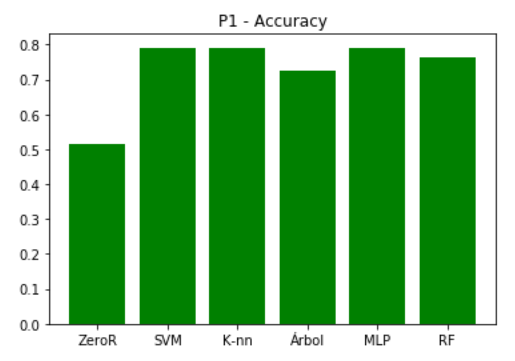
\includegraphics[width=43mm]{imagenes/p1_acc}}
  \subfigure[F1-Score]{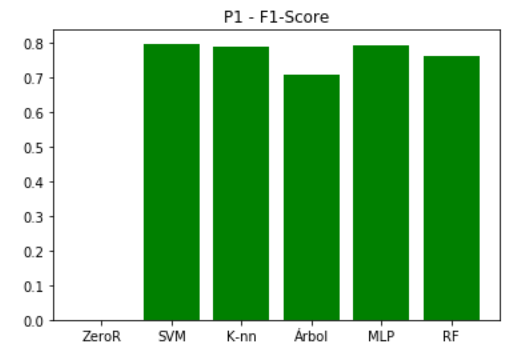
\includegraphics[width=43mm]{imagenes/p1_f1}}
  \subfigure[TPR]{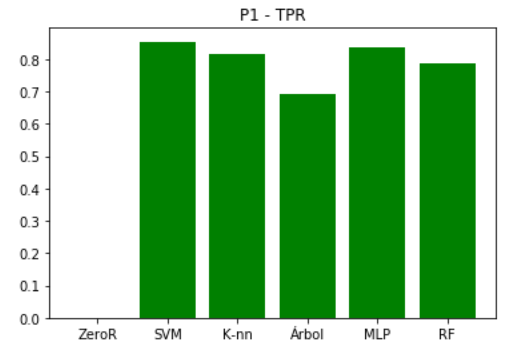
\includegraphics[width=43mm]{imagenes/p1_tpr}}
  \subfigure[FNR]{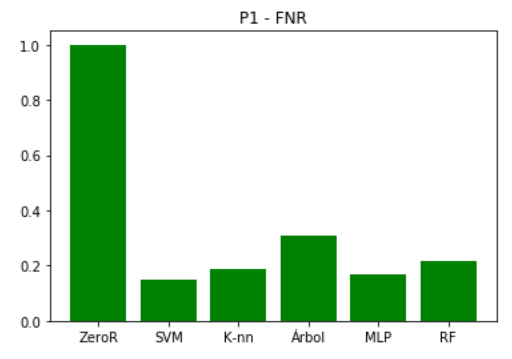
\includegraphics[width=43mm]{imagenes/p1_fnr}}
\end{figure}

\vspace{-5mm}

\begin{center}
  \textbf{Procesado 2}
\end{center}

\begin{figure}[H]
  \centering
  \subfigure[Accuracy]{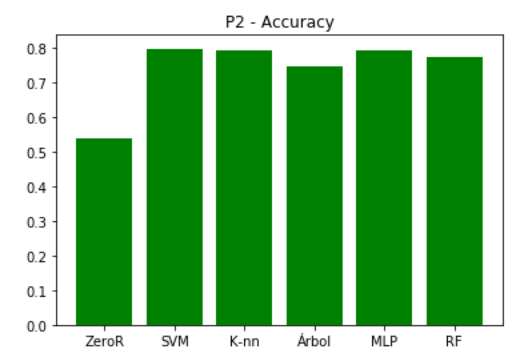
\includegraphics[width=43mm]{imagenes/p2_acc}}
  \subfigure[F1-Score]{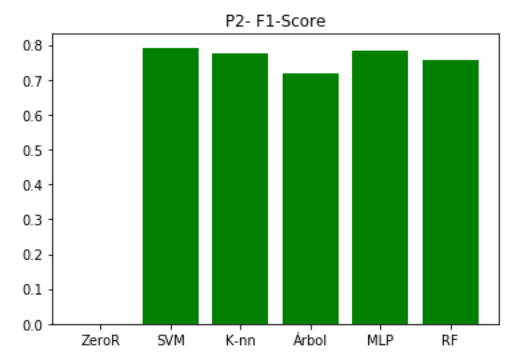
\includegraphics[width=43mm]{imagenes/p2_f1}}
  \subfigure[TPR]{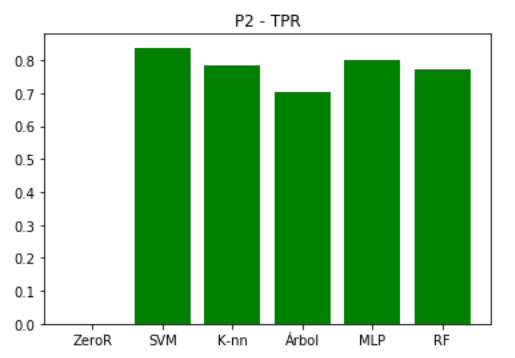
\includegraphics[width=43mm]{imagenes/p2_tpr}}
  \subfigure[FNR]{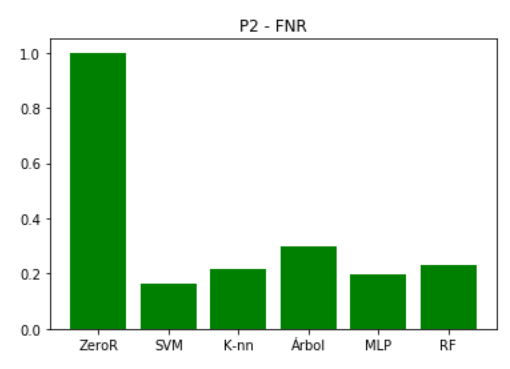
\includegraphics[width=43mm]{imagenes/p2_fnr}}
\end{figure}

\vspace{-5mm}

\begin{center}
  \textbf{Procesado 3}
\end{center}

\begin{figure}[H]
  \centering
  \subfigure[Accuracy]{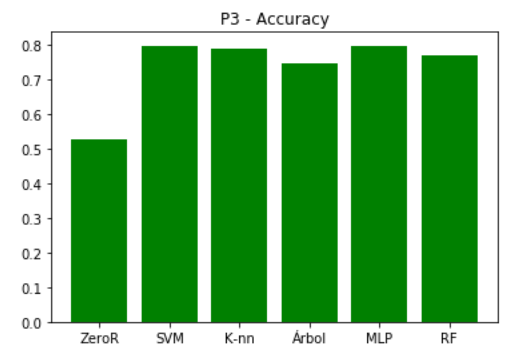
\includegraphics[width=43mm]{imagenes/p3_acc}}
  \subfigure[F1-Score]{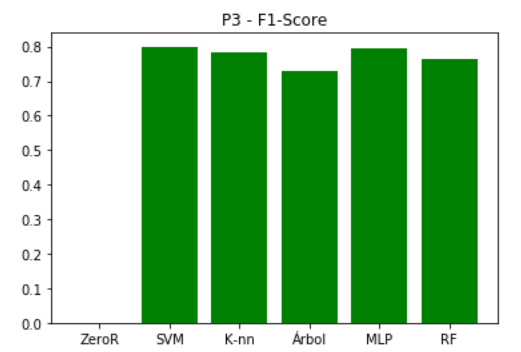
\includegraphics[width=43mm]{imagenes/p3_f1}}
  \subfigure[TPR]{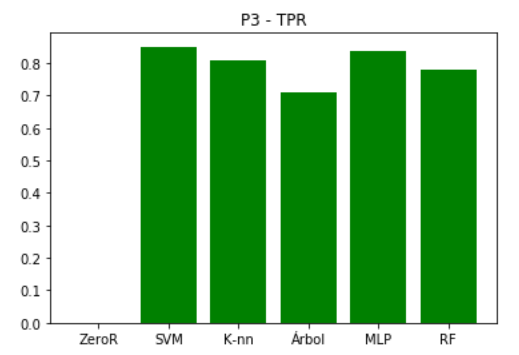
\includegraphics[width=43mm]{imagenes/p3_tpr}}
  \subfigure[FNR]{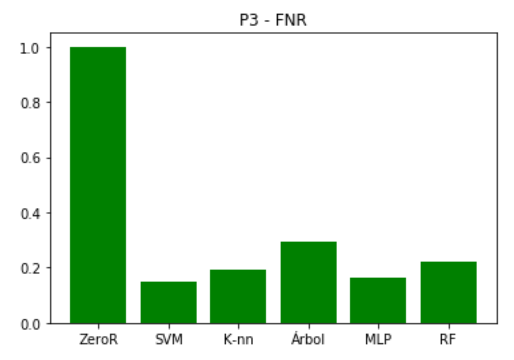
\includegraphics[width=43mm]{imagenes/p3_fnr}}
\end{figure}

\vspace{-5mm}

El código de cada gráfica es:

\begin{lstlisting}
fig, ax = plt.subplots()
ax.bar(["ZeroR", "SVM", "K-nn", "Arbol", "MLP", "RF"], pX_metrica, color='green')
ax.set_title("PX-metrica")
\end{lstlisting}

Donde ``X'' es denota el preprocesado que se ha aplicado, $1, 2$ o $3$, y `` metrica'' la métrica que se mide, pudiendo ser \texttt{accuracy}, \texttt{F1-Score}, \texttt{TPR} o \texttt{FNR}. El vector pX-metrica es un vector donde se guardan los valores de la métrica ``metrica'' con el preprocesado ``X'' de todos los modelos considerados.

Podemos observar que los tres preprocesados obtienen resultados muy similares, como ya comentamos en la práctica anterior. A primera vista, la estructura de los diagramas parece la misma, es decir, al ordenar los diferentes modelos según el valor de la métrica correspondiente con cada procesamiento, este orden es muy parecido en todos ellos, no atreviéndome a decir el mismo por haber barras de alturas semejantes. Es por esto que decantarse por un procesamiento con estos gráficos resulta complicado.

En los tres preprocesamientos el modelo con menor \texttt{accuracy} es el ZeroR, seguido del árbol de decisión. El SVM, K-nn y MLP son los modelos con mayor \texttt{accuracy} en los tres casos. En el resto de métricas se obserba que el SVM y el MLP tienen un mejor desempeño que el K-nn, siendo estos dos modelos los que mejores resultados obtienen. El árbol de decisión y el ZeroR son los modelos que peor desempeño tienen. El Random Forest y el árbol de decisión no obtienen tan buenos resultados como los otros modelos inicialmente pero, como vimos en la práctica 1, aplicando la poda coste-complejidad obteniamos una gran mejora de su desempeño, ya que con esta poda se conseguía reducir el sobreajuste del modelo.

Para elegir que procesamiento utilizabamos en la práctica 1, nos decantamos por el procesamiento que en más modelos tuviese mayor \texttt{F1-Score}. En las siguientes gráficas mostramos el valor de esta métrica en los diferentes modelos para cada procesamiento: 

\begin{figure}[H]
  \centering
  \subfigure[ZeroR]{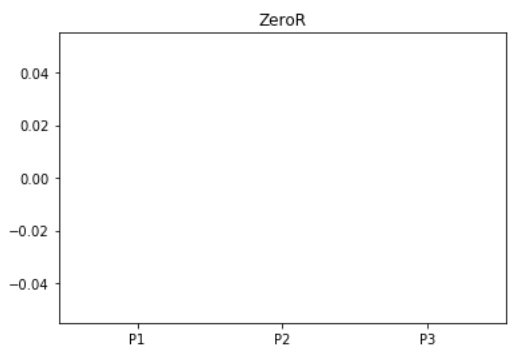
\includegraphics[width=57mm]{imagenes/zeror}}
  \subfigure[SVM]{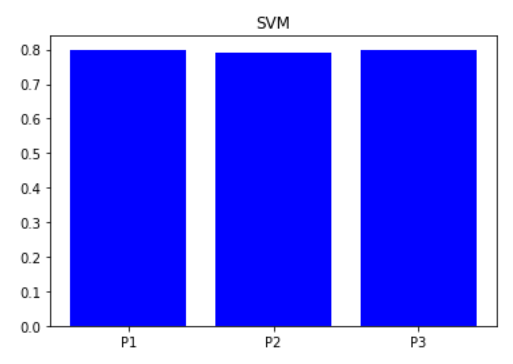
\includegraphics[width=57mm]{imagenes/svm}}
  \subfigure[k-nn]{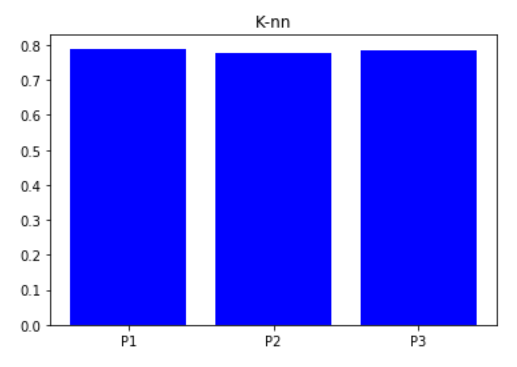
\includegraphics[width=57mm]{imagenes/knn}}
\end{figure}

\begin{figure}[H]
  \centering
  \subfigure[Árbol de decisión]{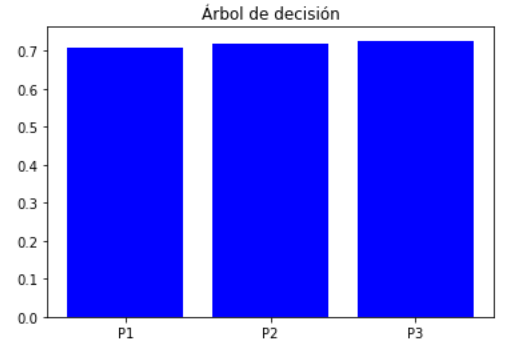
\includegraphics[width=58mm]{imagenes/arbol}}
  \subfigure[MLP]{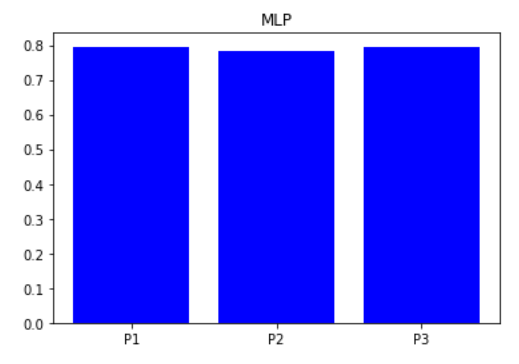
\includegraphics[width=55mm]{imagenes/mlp}}
  \subfigure[Random Forest]{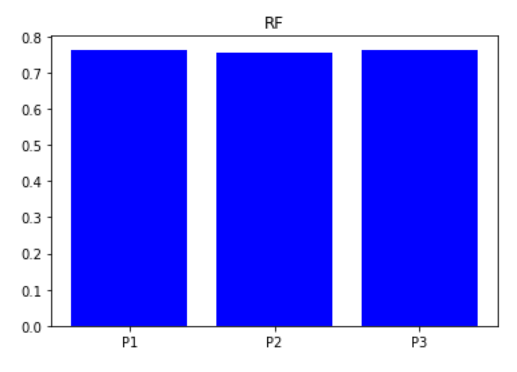
\includegraphics[width=60mm]{imagenes/rf}}
\end{figure}

Como ya hemos visto antes, no hay gran diferencia entre unos y otros. En el modelo ZeroR la \texttt{F1-Score} es $0$ en los tres casos, debido a que etiqueta todas las muestras como negaticas, luego no hay verdaderos positivos. En los modelos SVM, MLP, Random Forest y K-nn el procesamiento de datos 2 parece tener resultados ligeramente inferiores que los otros dos, que están muy igualados. En el árbol de decisión el procesamiento 2 tiene un mejor desempeño que el 1, pero peor que el 3. Este modelo es el que peores resultados ofrece sin considerar el ZeroR. Como podemos obsservar que el eje $Y$ no llega a $0.8$ como en los demás.

Al igual que en la práctica 1, el procesado de datos  que usaría usando la información recogida en estas gráficas sería el procesado 3, porque en el árbol de decisión se ve que es el que mejores resultados ofrece y en el resto de modelos la diferencia con el procesado 1 no puedo apreciarla a simple vista.

Para crear las gráficas primero se crearon para cada modelo vector que contiene el valor de la métrica \texttt{F1-Score} de cada uno de los preprocesados:

\begin{lstlisting}
v_zeror = [p1_f1[0], p2_f1[0], p3_f1[0]]
v_svm   = [p1_f1[1], p2_f1[1], p3_f1[1]]
v_knn   = [p1_f1[2], p2_f1[2], p3_f1[2]]
v_arbol = [p1_f1[3], p2_f1[3], p3_f1[3]]
v_mlp   = [p1_f1[4], p2_f1[4], p3_f1[4]]
v_rf    = [p1_f1[5], p2_f1[5], p3_f1[5]]
\end{lstlisting}

Tras esto, para cada uno de los modelos creamos la gráfica correspondiente así:

\begin{lstlisting}
fig, ax = plt.subplots()
ax.bar(["P1", "P2", "P3"], v_clf, color='blue')
ax.set_title("clf")
\end{lstlisting}

donde ``clf'' denota el clasificador del que recogemos los datos en la gráfica.  

\subsection{Curva ROC}

Para representar la curva ROC dividimos el conjunto de datos al que se le ha aplicado el procesado 3 salvo la normalización en comjunto de entrenamiento y conjunto de validación. La división se hace de manera que el $70\%$ de los datos formen el conjunto de entrenamiento y el otro $30\%$, el de test, conservando la proporción de elementos en cada clase tanto en el conjunto de entrenamiento como en el de validación. Esto se hace con el código:

\begin{lstlisting}
  X_train, X_test, y_train, y_test = model_selection.train_test_split(data, target,
  test_size=0.3, stratify=target, random_state=0)
\end{lstlisting}

Tras esto,, completamos el procesado de datos $3$ usando \texttt{MinMaxScaler()} para normalizar los datos de entrenamiento y se usa estas mismas transformaciones sobre los datos de validación. A continuación, entrené los modelos con los hiperparámetros seleccionados en la práctica anterior. Podemos representar en una gráfica la curva ROC de los diferentes modelos así:

\begin{lstlisting}
ax = plt.gca()

for model in [dummy_clf, svm_clf, knn_clf, tree_clf, mlp_clf, rf_clf]:
    metrics.plot_roc_curve(model, data, target, ax=ax)  
\end{lstlisting}

El resultado es:

\begin{figure}[H]
  \centering
  \caption{Curva ROC}
  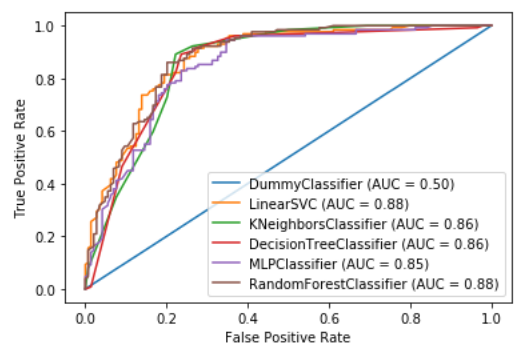
\includegraphics[width=131mm]{imagenes/ROC}
\end{figure}

Los modelos que presentan mayor métrica \texttt{AUC} son el Random Forest y el SVM, que son aquellos con mayor área bajo la curva ROC y los que tienen una mayor pendiente en los valores cercanos al cero. Esto implica que estos clasificadores son capaces de incrementar el número de verdaderos positivos a un ritmo mayor que el número de falsos positivos. Si usásemos esta métrica para sacar conclusiones, éstos serían los mejores modelos, mientras que el  MLP es el modelo que peor comportamiento muestra, excluyendo al ZeroR. A pesar de esto, no hay excesivas diferencias entre los modelos considerados, a excepción del ZeroR.

\subsection{Análisis de los atributos}

En esta sección estudiaremos la importancia de los diferentes atributos en la clasificación. Para ello se visualizarán gráficos de barras para cada uno de los diferentes atributos y para cada una de las etiquetas, de manera que se muestre la distribución de los valores que toma dicho atributo en función de su etiqueta. También visualizaremos los diagramas de cajas, ``boxplots'', de aquellos atributos donde tenga sentido.\\

Empezamos mostrando las gráficas correspondientes al atributo \texttt{BI-RADS}:

\begin{figure}[H]
  \centering
  \caption{Cantidad de datos con cada etiqueta}
  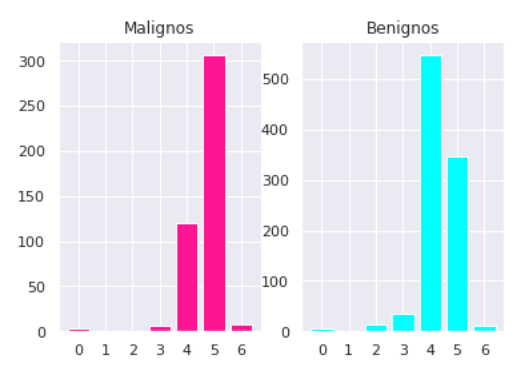
\includegraphics[width=100mm]{imagenes/bi_rads}
\end{figure}

Este atributo representa la opinión de un médico experto sobre la gravedad del tumor. Si tiene el valor ``1'' o ``2'', el tumor es benigno, del mismo modo, si toma el valor ``6'' es maligno. Los valores ``3'', ``4'' y ``5'' designan casos en los que no se está seguro de la severidad del tumor, pero hay cierta probabilidad de que sea maligno o benigno. Esta información la podemos comprobar en \href{https://es.wikipedia.org/wiki/BI-RADS}{https://es.wikipedia.org/wiki/BI-RADS}. Este atributo da mucha información sobre la naturaleza del tumor, pero dado que necesitamos la opinión de un experto para obtenerlo, no es apropiado usarlo para el aprendizaje.

Según la página \href{https://bigml.com/user/TotyB/gallery/dataset/509a98c6035d0706dd0001dd}{https://bigml.com/user/TotyB/gallery/dataset/509a98c6035d0706dd0001dd}, de donde hemos obtenido los datos, el $94.46\%$ de estos tienen \texttt{BI-RADS} ``4'' o ``5''. De estos, los tumores con valor ``5'' son probablemente malignos. Los tumores malignos tienen más variabilidad que los benignos, dado que hay tumores malignos con valor de \texttt{BI-RADS} ``4'' o ``5'', predominando el valor ``5''. En el caso de los benignos, la mayoría de estos tienen la categoría de \texttt{BI-RADS} ``4''.

Esto se ve en el diagrama de cajas de este atributo:

\begin{figure}[H]
  \centering
  \caption{Diagrama de cajas de BI-RADS}
  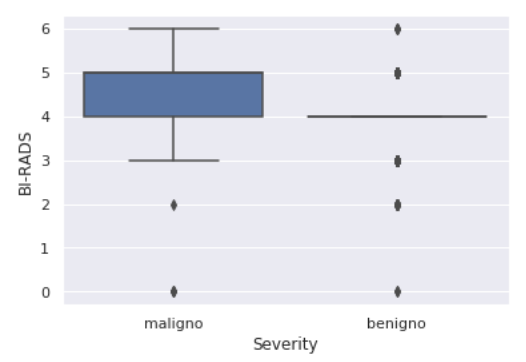
\includegraphics[width=100mm]{imagenes/bp_birads}
\end{figure}

Los tumores etiquetados como malignos se mueven entre el valor ``4'' o ``5'' mientras que la mayoría de los benignos toman el valor ``4''.

La gráfica del atributo edad nos proporciona los siguientes resultados:

\begin{figure}[H]
  \centering
  \caption{Cantidad de datos con cada etiqueta}
  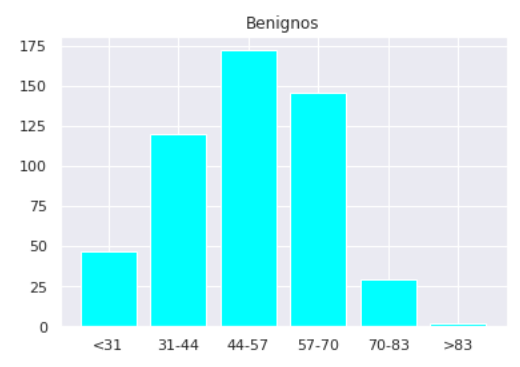
\includegraphics[width=87mm]{imagenes/edad_ben}
  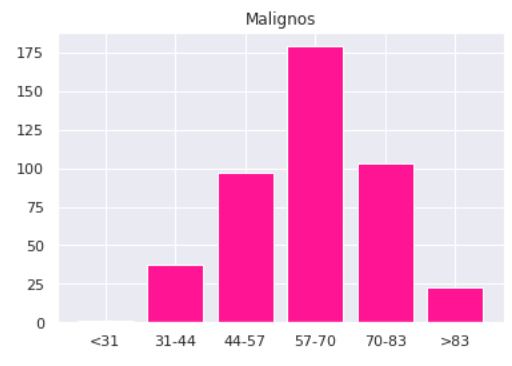
\includegraphics[width=87mm]{imagenes/edad_mal}
\end{figure}

Vemos que cuanto menor edad tiene una persona, más probable es que su tumor sea benigno. En particular, la mayoría de las personas menores de $31$ años de la muestra tienen tumores benignos y gran parte de las que tienen más de $83$ tienen tumores malignos. En el diagrama de cajas podemos observar que la mediana de edad de los pacientes con tumores malignos de la muestra es superior a los $60$ años, mientras que la de los pacientes con tumores benignos está rondando los $50$. Aunque la edad de los pacientes con tumores benignos varía entre los $18$ y algo más de los $80$ años, los datos entre el primer y el tercer cuartil se encuentran concentrados entre los $40$ y $60$. Los datos entre el primer y el tercer cuartil de los tumores malignos se encuentran entre algo más de los $50$ y algo más de los $70$ años.

Por consiguiente, la edad de una persona sí es un atributo relevamte en la clasificación, porque aunque no podríamos estimar la severidad del tumor sabiendo sólo la edad de ésta, si una persona es muy joven podríamos esperar que su tumor sea benigno. 

\begin{figure}[H]
  \centering
  \caption{Diagrama de cajas de la edad}
  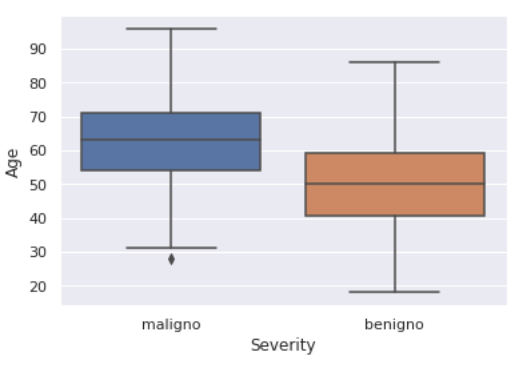
\includegraphics[width=87mm]{imagenes/bp_age}
\end{figure}

A continuación, analizaremos las gráficas del atributo Shape. La mayoría de los tumores malignos tienen una forma irregular, mientras que los benignos suelen tener una forma ovalada o redondeada. Los tumores benignos presentan mayor variabilidad en los valores que toman en este atributo que los malignos. Resulta interesante considerar este atributo para nuestro aprendizaje, ya que la distribución de los valores que toman los tumores malignos difiere bastante de la de los benignos.\\

\begin{figure}[H]
  \centering
  \caption{Cantidad de datos con cada etiqueta}
  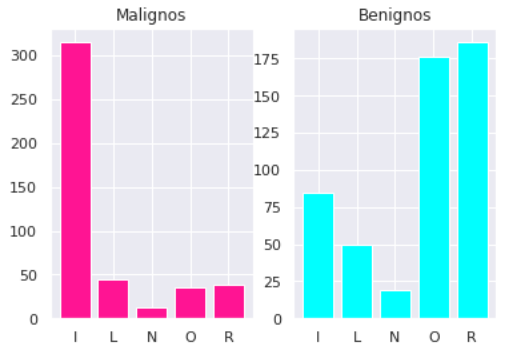
\includegraphics[width=87mm]{imagenes/shape}
\end{figure}

Como el atributo Shape es cualitativo y no tiene orden, no tiene sentido dibujar un diagrama de cajas en este caso, ya que este variaría para cada asignación diferente de valores numéricos a cada posible valor del atributo, y esta asignación es totalmente aleatoria, ya que estos carecen de orden.\\

El siguiente atributo a analizar es Margin. Al igual que en Shape, los distintos valores que toma este atributo no tienen un orden determinado, por lo tanto no representé el diagrama de cajas de este atributo. Los tumores malignos tienen mayor variabilidad que los benignos, siendo el valor de Margin más frecuente entre estos ``ill-defined'' seguido del ``spiculated''. Los benignos, sin embargo, suelen tener margin ``circumscribed''. En la práctica 1, una vez eliminados los atributos \texttt{BI-RADS} y Density, vimos que este atributo era el que mayor información nos aportaba en la clasificación, dado que era el elegido en el nodo raíz del árbol de decisión. Aquí podemos comprobar que efectivamente hay una gran diferencia entre la distribución de los valores de Margin que toman los tumores malignos de los benignos, cosa que afecta favorablemente a la clasificación, permitiéndonos diferenciar una muestra maligna de una benigna con mayor facilidad.

\begin{figure}[H]
  \centering
  \caption{Cantidad de datos con cada etiqueta}
  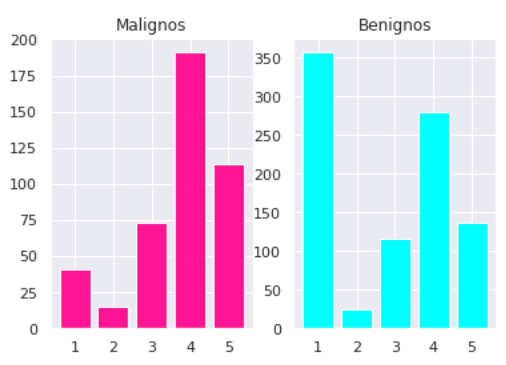
\includegraphics[width=87mm]{imagenes/margin}
\end{figure}

Por último, analizamos el atributo Density. Como ya comentamos, este atributo tiene muy poca variabilidad en la muestra y podemos comprobar que los dos diagramas de barras son muy parecidos, lo que nos incita a pensar que este atributo no aporta apenas información a la clasificación.

\begin{figure}[H]
  \centering
  \caption{Cantidad de datos con cada etiqueta}
  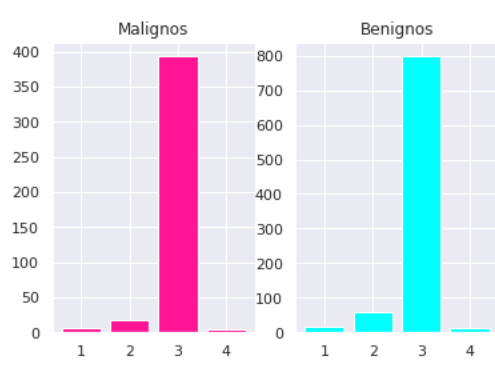
\includegraphics[width=87mm]{imagenes/density}
\end{figure}

En el diagrama de cajas volvemos a apreciar la poca variabilidad de este atributo, ya que cualquier valor distinto de $3$ lo interpreta como outlayer. Esta razón fue la que me llevó a considerar eliminar este atributo durante el procesado de datos $3$.

\begin{figure}[H]
  \centering
  \caption{Diagrama de cajas de Density}
  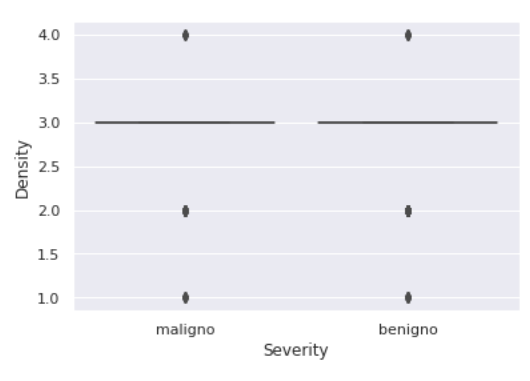
\includegraphics[width=65mm]{imagenes/bp_density}
\end{figure}

\section{Segmentación}

\subsection{Introducción}

El problema que abordaremos en esta sección es agrupar accidentes obtenidos de los datos publicados por la Dirección General de Tráfico  en conjuntos de accidentes con características similares. Para ello utilizaremos técnicas de clustering estudiadas en la asignatura, concretamente \texttt{K-means} y \texttt{DBSCAN}. Ambos métodos son métodos de particionamiento.

El algortimo \texttt{K-means} necesita como parámetro el número de clústers deseado y va clasificando las diferentes instancias en el clúster cuyo centroide sea el más cercano a ésta. Es un método iterativo que recalcula el centroide en cada iteración y repite el proceso de clasificación de las instancias. Termina cuando en una iteración ninguna instancia cambia de clúster. El algoritmo siempre converge.

El algoritmo \texttt{DBSCAN} depende de los parámetros \textit{epsilon} y \textit{min\_samples}. El primero indica la distancia máxima a la que se considera que dos puntos son directamente alcanzables. Para que un punto sea un punto núcleo necesita que haya al menos \textit{min\_samples} a distancia menor que \textit{epsilon} de él. A partir de ahí, un punto será alcanzable si existe una secuencia de puntos $p_1, \ldots, p_n$ tales que $p_{i+1}$ es directamente alcanzable desde $p_i$. Cada punto núcleo forma un clúster formado por todos aquellos puntos alcanzables desde él. A los puntos que no pertenecen a ningún clúster se les asigna el clister $-1$.

Los atributos en los que nos basamos para hacer la segmentación son:

\begin{itemize}
\item \texttt{TOT\_VICTIMAS}: Total de víctimas
\item \texttt{TOT\_MUERTOS}: Total de muertos
\item \texttt{TOT\_HERIDOS\_GRAVES}: Total de heridos graves.
\item \texttt{TOT\_HERIDOS\_LEVES}: Total de heridos leves.
\item \texttt{TOT\_VEHICULOS\_IMPLICADOS}: Total de vehículos involucrados en el accidente.
\end{itemize}

Las métricas que usaremos para la estimar la bondad del ajuste son el coeficiente Silhouette y el índice Calinski-Harabasz.

El coeficiente Silhouette mide como de similares son los elementos del mismo clúster comparado con los elementos de otro clúster. Este coeficiente es la media de los $s(i)$, con

$$s(i) = \frac{b(i)-a(i)}{\max\{a(i), b(i)\}}$$

donde $b(i)$ es la mínima distancia del elemento $i$ a otro clúster y $a(i)$ es la distancia media del elemento al resto de instancias de su clúster. Cuanto mayor sea este coeficiente, mejor es el rendimiento del modelo.

El índice Calinski-Harabasz mide la razón entre la dispersión interclústers y la dispersión intraclústers. El agrupamiento será mejor cuanto mayor sea este índice.

Para la elección de hiperparámetros, elegiremos aquellos que maximicen el índice Calinski-Harabasz, que utiliza todas las muestras para su cálculo y dado que usamos los mismos datos en todas las iteraciones, que su valor no esté normalizado no afecta en la interpretación del resultado.

Antes de realizar el análisis ejecutando los algoritmos de clusterig normalizamos los datos con la función \texttt{MinMaxScaler}.

\newpage
\subsection{Caso de estudio 1: Choque frontal en carreteras convencionales}

Estudiaremos las propiedades de los choques frontal en carreteras convencionales que, según el libro \href{https://www.todostuslibros.com/libros/manual-del-alumno-permiso-b-facilauto_978-84-09-08551-4}{Manual del alumno. Permiso B} es el caso de accidente con más víctimas mortales.

\subsubsection{K-means}

El algoritmo \texttt{K-means} tiene como parámetro el número de clúster a considerar. Para elegir el mejor valor de éste, ejecuté el algoritmo con un número de clústers comprendido entre $2$ y $14$. Los resultados de las métricas son:

\begin{center}
\begin{tabular}{|c|c|c|}
\hline
\multicolumn{1}{|c|}{\textbf{Nº de clústers}}& \textbf{Silhouette} & \textbf{Calinski-Harabasz}\\ \hline
  2  & 0.4755151052183165  & 637.8831140088855  \\ \hline
  3  & 0.46599969633063965 & 597.9798532808658  \\ \hline
  4  & 0.48348908673333896 & 634.4016355078425  \\ \hline
  5  & 0.531569055229591   & 683.2263367508311  \\ \hline
  6  & 0.5404576589330072  & 646.8004817570682  \\ \hline
  7  & 0.5519986909803548  & 630.8036708742871  \\ \hline
  8  & 0.5786471085948179  & 634.4445453990445  \\ \hline
  9  & 0.5903779353773022  & 628.3756258948337  \\ \hline
 10  & 0.6461326222918197  & 659.4342926638305  \\ \hline
 11  & 0.6893747693555886  & 653.852874658656   \\ \hline
 12  & 0.7336714808160643  & 659.3965542394021  \\ \hline
 13  & 0.744841516853055   & 665.0690582901761  \\ \hline
 14  & 0.749410469848095   & 663.5502144820157  \\ \hline
\end{tabular}
\end{center}

Para facilitar la comprensión de la tabla, visualizamos la información que contiene en las siguientes gráficas, que se realizan utilizando la función \texttt{grafica}, cuyo código es:

\begin{lstlisting}
def grafica(data, label, title, xlab, ylab):
    plt.plot(data,label, c='b')
    plt.title(title)
    plt.xlabel(xlab)
    plt.ylabel(ylab)

    plt.show()
  \end{lstlisting}

Obtenemos el siguiente resultado:

\begin{figure}[H]
  \centering
  \caption{Gráficas con el valor de las métricas en función del número de clústers}
  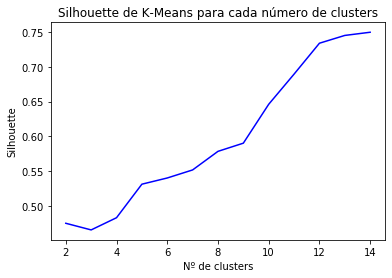
\includegraphics[width=87mm]{imagenes/c1_kmeans_sil}
  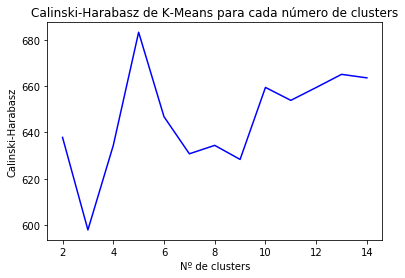
\includegraphics[width=87mm]{imagenes/c1_kmeans_cal}
\end{figure}

Vemos que el coeficiente Calinski-Harabasz alcanza un máximo cuando se consideran 5 clústers, por lo que elegiremos este valor para dicho hiperparámetro.

El resultado de la segmentación es la división del conjunto de accidentes considerados en 5 conjuntos con las siguiente distribución:

\begin{figure}[H]
  \centering
  \caption{Clústers}
  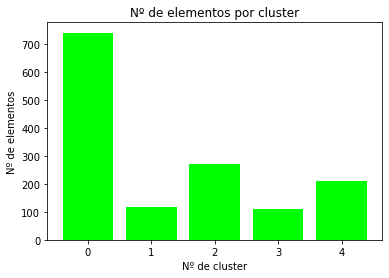
\includegraphics[width=100mm]{imagenes/c1_kmeans_clusters}
\end{figure}

Vemos que el $51.24\%$ de los accidentes pertenecen al clúster $0$. El siguiente clúster más grande, el $2$, posee el $18.65\%$ de éstos y el $4$ posee el $14.51\%$. Los clústers con menos elementos son el $1$ y el $3$ con el $8.08\%$ y el $7.53\%$, respectivamente.

Los valores de las métricas para este modelo son:

\begin{center}
\begin{tabular}{|c|c|}
\hline
\multicolumn{1}{|c|}{\textbf{Silhouette}} & \textbf{Calinski-Harabasz}\\ \hline
 0.531569055229591   & 683.2263367508311  \\ \hline
\end{tabular}
\end{center}

Los centroides de los diferentes clusters son:

\begin{figure}[H]
  \centering
  \caption{Centroides}
  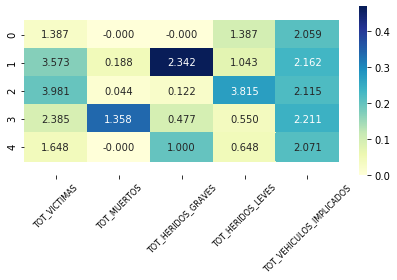
\includegraphics[width=130mm]{imagenes/c1_kmeans_centroides}
\end{figure}

El clúster $0$, que es aquel con más instancias, tiene como centro un accidente con $2.059$ vehículos implicados, del que $1.387$ personas han sido heridos leves, pero sin muertos ni heridos graves. Es el clúster cuyo centro tiene un menor número de víctimas.

El clúster $1$ tiene como centro un accidente con $3,573$ víctimas, en el que $2,342$ son heridos graves, $1.043$ son heridos leves y $0.188$ son heridos leves. Hubo $2.162$ vehículos implicados. Es el clúster con mayor número de heridos graves de media.

El clúster $2$ tiene como centro un accidente con $3.981$ víctimas, la mayoría heridos leves. Tiene de media más heridos leves que el resto, pero es el sugundo con menos heridos graves. Como en el resto de clústers, los vehículos involucrados están alrededor de $2$.

El clúster $3$ tiene como centro un accidente con $2.3850$ víctimas. Tiene de media más muertos que el resto, $1.358$ muertos. También tiene $0.477$ heridos graves y 0.55 heridos leves.

El cúster 4 tiene como centro un accidente con $1.648$ víctimas, pero ningún muerto.

Las diferencias entre los distintos clústers pueden visualizarse con \texttt{pairplot}:

\begin{figure}[H]
  \centering
  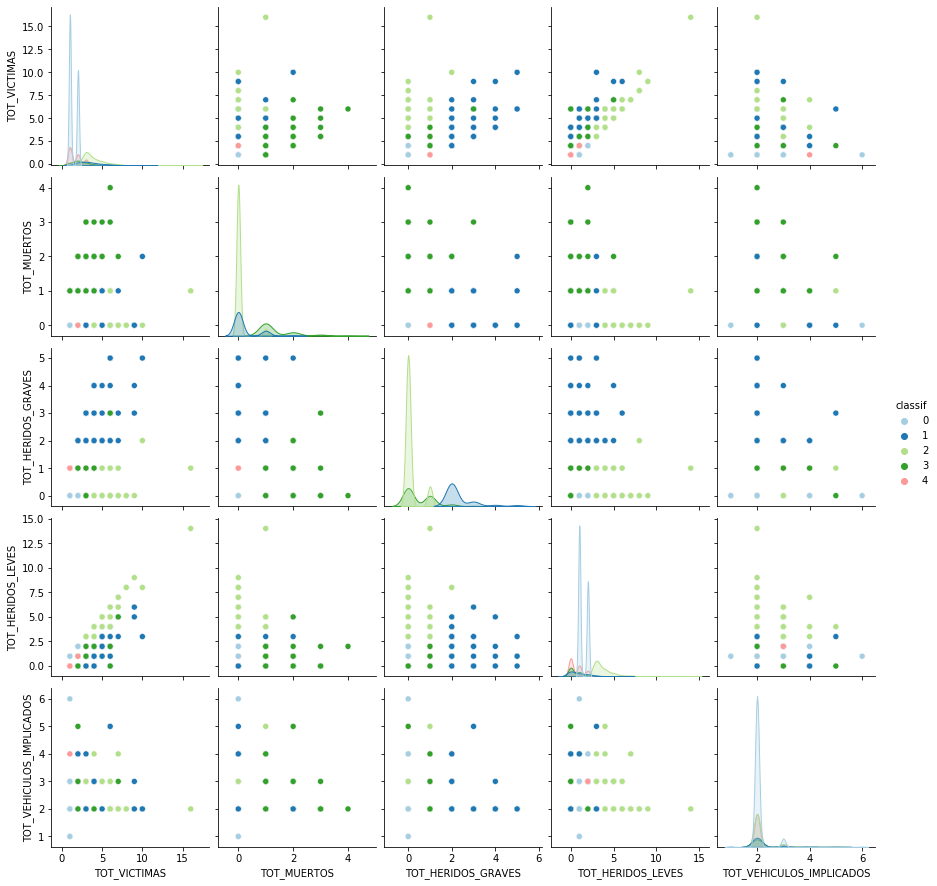
\includegraphics[width=171mm]{imagenes/c1_kmeans_pairplot}
\end{figure}

Podemos corroborar lo que vimos con los centroides, que todos los clústers suelen tener entorno a 2 vehículos implicados. En el atributo \texttt{TOT\_HERIDOS\_GRAVES} nos ayuda a discernir el clúster 1 de los clusters 2 y 3. El atributo \texttt{TOT\_HERIDOS\_LEVES} diferencia los clústers 4, 0 y 2. Para ver estas diferencias de manera más detallada podemos usar \texttt{boxplot}:

\begin{figure}[H]
  \centering
  \caption{Diagramas de cajas}
  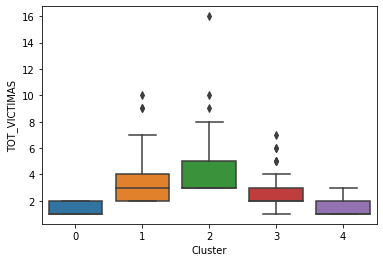
\includegraphics[width=87mm]{imagenes/c1_kmeans_bp_vic}
  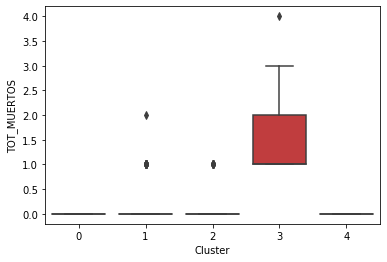
\includegraphics[width=87mm]{imagenes/c1_kmeans_bp_muertos}
    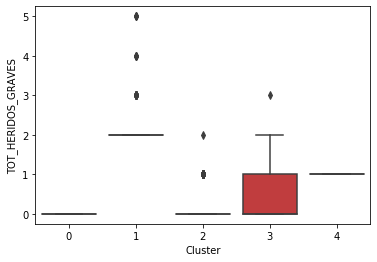
\includegraphics[width=87mm]{imagenes/c1_kmeans_bp_hg}
  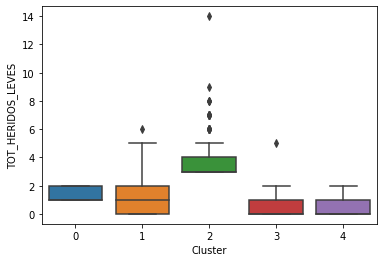
\includegraphics[width=87mm]{imagenes/c1_kmeans_bp_hl}
  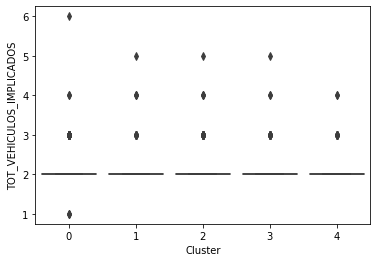
\includegraphics[width=87mm]{imagenes/c1_kmeans_bp_vi}
\end{figure}

\newpage
En la siguiente tabla mostramos el rango de valores más representativo de cada cluster:

\begin{center}
\begin{tabular}{|c|c|c|c|c|c|}
\hline
\multicolumn{1}{|c|}{\textbf{Nº del clúster}} & \textbf{Víctimas} & \textbf{Muertos} & \textbf{Heridos graves} & \textbf{Heridos leves} & \textbf{Vehículos implicados}\\ \hline
  0  & 0-2 & 0   & 0   & 1-2 & 2 \\ \hline
  1  & 2-7 & 0   & 2   & 0-5 & 2 \\ \hline
  2  & 3-8 & 0   & 0   & 3-5 & 2 \\ \hline
  3  & 0-4 & 1-3 & 0-2 & 1-2 & 2 \\ \hline
  4  & 0-3 & 0   & 1   & 1-2 & 2 \\ \hline
\end{tabular}
\end{center}

\newpage
\section{Contenido adicional}
\section{Bibliografía}

\textbf{Visualización}
\begin{itemize}
\item \href{https://es.wikipedia.org/wiki/BI-RADS}{https://es.wikipedia.org/wiki/BI-RADS}
\item Datos: \href{https://bigml.com/user/TotyB/gallery/dataset/509a98c6035d0706dd0001dd}{https://bigml.com/user/TotyB/gallery/dataset/509a98c6035d0706dd0001dd}
\end{itemize}
\textbf{Segmentación}
\begin{itemize}
\item Transparencias Tema 5: Clustering
\item \href{https://www.todostuslibros.com/libros/manual-del-alumno-permiso-b-facilauto_978-84-09-08551-4}{Manual del alumno. Permiso B}
\item \href{https://github.com/SofiaAlmeida/IN/blob/master/P2/memoria.pdf}{https://github.com/SofiaAlmeida/IN/blob/master/P2/memoria.pdf}
\item \href{https://scikit-learn.org/stable/modules/generated/sklearn.cluster.KMeans.html\#sklearn.cluster.KMeans.fit}{https://scikit-learn.org/stable/modules/generated/sklearn.cluster.KMeans.html\#sklearn.cluster.KMeans.fit}
\item \href{https://scikit-learn.org/stable/modules/generated/sklearn.cluster.DBSCAN.html\#sklearn.cluster.DBSCAN}{https://scikit-learn.org/stable/modules/generated/sklearn.cluster.DBSCAN.html\#sklearn.cluster.DBSCAN}
\item \href{https://es.wikipedia.org/wiki/DBSCAN}{https://es.wikipedia.org/wiki/DBSCAN}
\end{itemize}

\end{document}
